 \chapter{Numerical Experiments}

\section{Investigation of temporal stability}

Preliminary work regarding discretization and numerical analysis of the second order Crank-Nicholson time stepping scheme for fluid structure interaction can be found in \cite{Wickb}. Two main properties of interest 
 have proven to be the stability of long-time simulation, and obtaining the expected physics for the problem of interest. One of the main challenges for constructing time-stepping schemes for ALE-methods, is the additional non-linearity introduced by the domain-velocity term in the fluid problem. 

\begin{align}
\ha{J} (\hat{F}_f^{-1}(\bat{v} - \pder{\ha{T}_f}{t}) \cdot \hat{\nabla}) \bat{v}
\end{align} 

The stability of first and second-order time stepping schemes for ALE-methods have proven to be affected by the ALE-convection term  \cite{Formaggia2004, Formaggia1991}, but to what extent remains unclear. Closer inspection of the convection term reviles spatial and temporal differential operators depending non-linearly on one another. These differential operators often appear separated, making discretization of a general time-stepping scheme is not directly intuitive, and often based on the experience of similar equations such as the Navier-Stokes equations. \\

The Crank-Nicolson scheme can suffer from temporal stability for long-term simulations \cite{Wick2013a}. Therefore,the authors of \cite{Richter2015}, investigated temporal stability of the Crank-Nicolson scheme for the validation benchmark found in \cite{Hron2006}.  
The criteria for the numerical experiments was to obtain a stable solution in the time interval [0, 10] minutes, by temporal and spatial refinement studies. The fully monolithic FSI problem discretized with second-order Crank-Nicolson, proved to give general stability problems for long-term simulation for certain time-steps \textit{k}.  Following the ideas of \cite{Richter2015},, a second order scheme based on the Cranck-Nicholson yields two possibilities.

\begin{discr}
\textit{Crank–Nicolson secant method }
\begin{align*}
\Big[\frac{\ha{J}(\bat{u}^{n}) \bat{\nabla} \bat{v}^{n} \bat{F}_W^{-1}}{2} 
+ \frac{\ha{J}(\bat{u}^{n-1}) \bat{\nabla} \bat{}v^{n-1} \bat{F}_W^{-1}}{2} \Big] 
\frac{\bat{u}^{n} - \bat{u}^{n-1}}{k}
\end{align*} 
\end{discr}

\begin{discr}
\textit{Crank–Nicolson midpoint-tangent method}
\begin{align*}
\Big[\frac{\ha{J}(\bat{u}_{cn}) \bat{\nabla} \bat{v}_{cn} \bat{F}_W^{-1}}{2} \Big] 
\frac{\bat{u}^{n} - \bat{u}^{n-1}}{k} \hspace{4mm}
\bat{u}_{cn} = \frac{\bat{u}^{n} + \bat{u}^{n-1}}{2} \hspace{2mm}
\bat{v}_{cn} = \frac{\bat{v}^{n} + \bat{v}^{n-1}}{2}
\end{align*} 
\end{discr}

The numerical experiments showed very similar performance for Discretization 1.1 and 1.2 , and significant differences of temporal accuracy was not found \cite{Richter2015}.  Two options to coupe with the presented unstabilities are the \textit{shifted Crank-Nicolson} \cite{Richter2015, Wicka, Wick2013a},   and the \textit{frac-step method}. Both of these methods are defined as A-stable time-stepping schemes meaning..  In this thesis the shifted Crank-Nocolson scheme was considered, introducing stability to the overall system by shifting the $\theta$ paramter slightly to the implicit side. If the shift is dependent of the time-step \textit{k} such that $\frac{1}{2} \leq \theta \leq \frac{1}{2} + k$, the scheme will be of second order \cite{Richter2015}.

\subsubsection*{Results}

\begin{figure}[h!]
 	\centering
    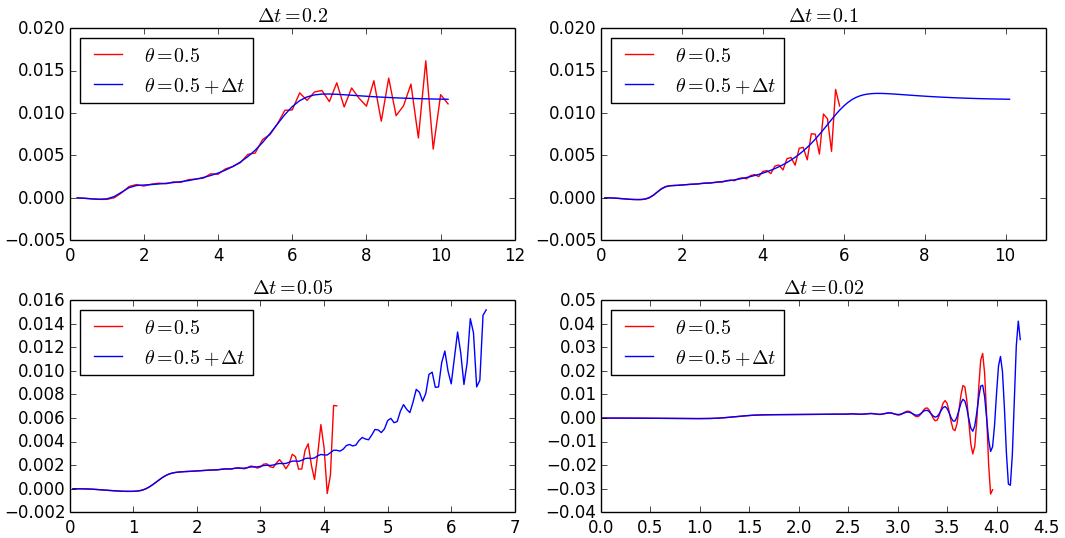
\includegraphics[scale=0.6]{./Fig/thetacheck.png} \\
      \caption{Investigation of temporal stability for the FSI3 benchbark in the time interval $t \in [0, 10]$, comparing the shifted crank nicolson to the original cranc nicolson scheme. }
\end{figure}

\newpage

\begin{figure}[h!]
 	\centering
    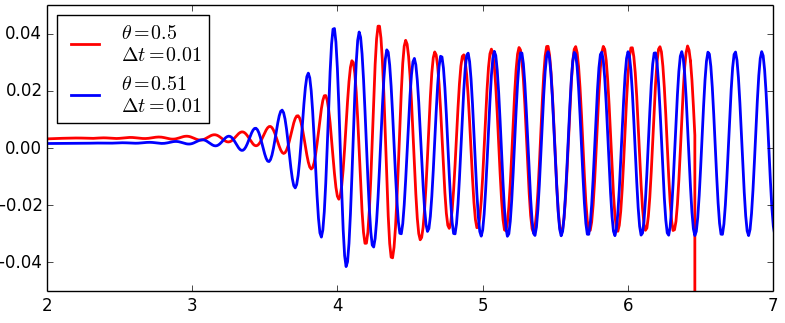
\includegraphics[scale=0.6]{./Fig/besttheta.png}
      \caption{Investigation of temporal stability for the FSI3 benchbark in the time interval $t \in [0, 10]$, comparing the shifted crank nicolson to the original cranc nicolson scheme. }
\end{figure}

A numerical investigation of temporal stability in shown in Figure 6.1-2, where the shifted crank-nicolson scheme $\theta = 0.5 + k$, is compared the original crank-nicolson $\theta = 0.5$. The shifted version clearly show stability properties surpassing the original crank-nicolson scheme, for all numerical experiments. However, for $\Delta t \in [0.2, 0.1, 0.05, 0.02]$ the scheme clearly lacks the ability to capture the overall physics of the validation problem. Long-time stability and expected physical beavior is obtained for $\Delta t = 0.01$. However, numerical experiments showed that for $\Delta t \leq 0.005$ numerical stability was achieved regardless of both methods. This result is important, reducing the overall computational time needed to achieve reasonable accuracy.


\newpage
\section{Optimization of Newtonsolver}
A \textit{bottleneck} express a phenomena where the total performance of a complete implementation is limited to small code fragments, accounting for the primary consumption of computer resources.

As for many other applications, within computational science one can often assume the consummation of resources follows the \textit{The Pareto principle}. Meaning that for different types of events, roughly 80\% of the effects come from 20\% of the causes. An analogy to computational sciences it that 80\% of the computational demanding operations comes from 20\% of the code. In our case, the bottleneck is the newtonsolver. The two main reasons for this is 

\begin{itemize}
\item \textbf{Jacobian assembly} \\
The construction of the Jacobian matrix for the total residue of the system, is the most time demanding operations within the whole computation. 
\item \textbf{Solver}. \\ 
As iterative solvers are limited for the solving of fluid-structure interaction problems, direct solvers was implemented for this thesis. As such, the operation of solving a linear problem at each iteration is computational demanding, leading to  less computational efficient operations. Mention order of iterations?
\end{itemize}

Facing these problems, several attempts was made to speed-up the implementation. The FEniCS project consist of several nonlinear solver backends, were fully user-customization option are available. However one main problem which we met was the fact that FEniCS assembles the matrix of the different variables over the whole mesh, even though the variable is only defined in one to the sub-domains of the system.In our case the pressure is only defined within the fluid domain, and therefore the matrix for the total residual consisted of several zero columns within the structure region. FEniCS provides a solution for such problems, but therefore we were forced to construct our own solver and not make use of the built-in nonlinear solvers. \\

The main effort of speed-up were explored around the Jacobian assembly.
Of the speed-ups methods explored in this thesis, some are \textit{consistent} while others are \textit{nonconsistent}. Consistent methods are methods that always will work, involving smarter approaches regarding the linear system to be solved. The non-consistent method presented involves altering the equation to be solved by some simplification of the system. As these simplifications will alter the expected convergence of the solver, one must take account for additional Newton iterations against cheaper Jacobi assembly. Therefore one also risk breakdown of the solver as the Newton iterations may not converge.   


\subsection{Consistent methods}
\subsubsection{Jacobi buffering}
By inspection of the Jacobi matrix, some terms of the total residue is linear terms, and remain constant within each time step. By assembling these terms only in the first Newton iteration will save some assembly time for the additional iterations needed each time step. As consequence the convergence of the Newton method should be unaffected as we do not alter the system.  

\subsection{Non-consisten methods}    
\subsubsection{Reuse of Jacobian}
As the assembly of the Jacobian at each iteration is costly, one approach of reusing the Jacobian for the linear system was proposed. In other words, the LU-factorization of the system is reused until the Jacobi is re-assembled. This method greatly reduced the computational time for each time step. By a user defined parameter, the number of iterations before a new assembly of the Jacobian matrix can be controlled. 

\subsubsection{Quadrature reduce}
The assemble time of the Jacobian greatly depends on the degree of polynomials used in the discretisation of the total residual. Within FEniCS t he order of polynomials representing the Jacobian can be adjusted. The use of lower order polynomials reduces assemble time of the matrix at each newton-iteration, however it leads to an inexact Jacobian which may results to additional iterations. 


\subsection{Comparison of speedup methods}

\begin{figure}[h!]
 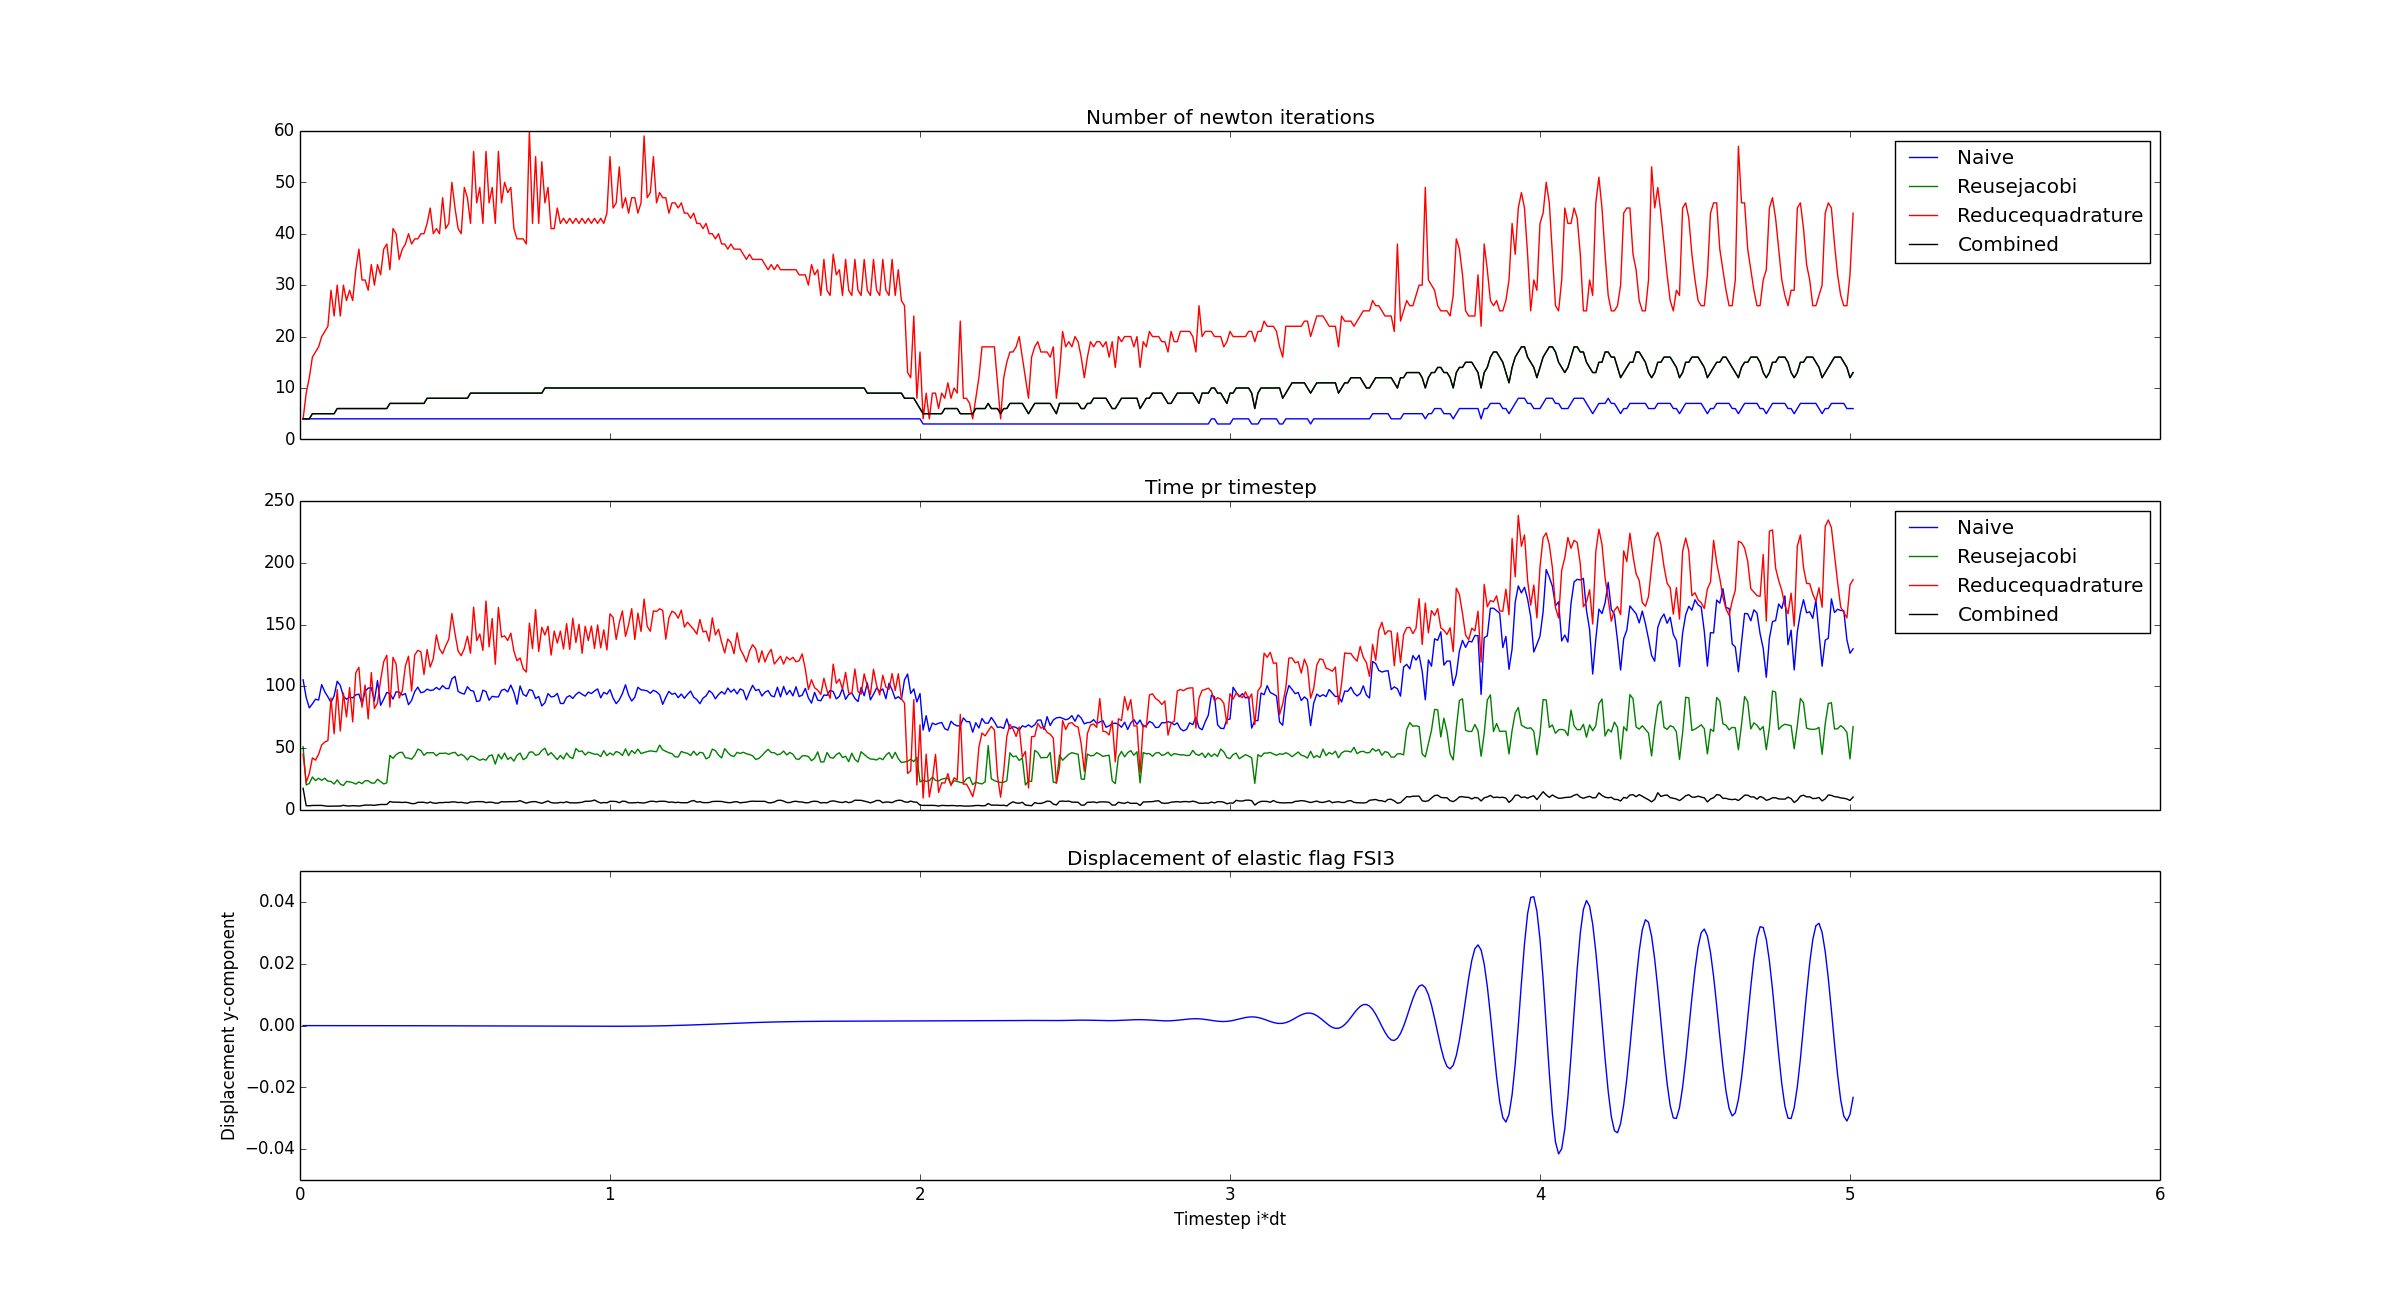
\includegraphics[scale=0.36]{./Fig/itercompare.png}
 \caption{Comparison of speed-up techniques for the laplace mesh model}
\end{figure}

\begin{figure}[h!]
 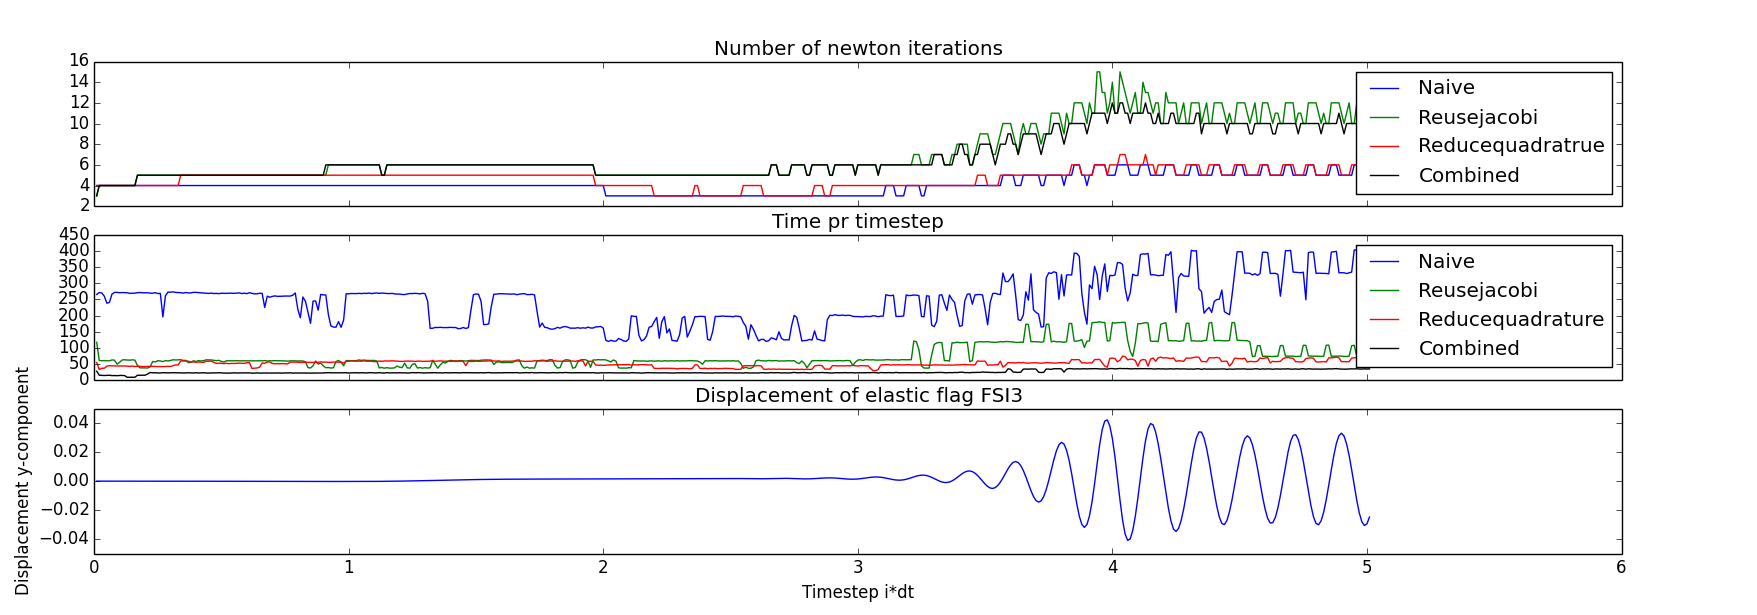
\includegraphics[scale=0.4]{./Fig/bi_compareit.png}
 \caption{Comparison of speed-up techniques for the biharmonic type 1 mesh model}
\end{figure}


\begin{table}[h!]
\centering
\caption{Comparison of speedup techniques}
\label{my-label}
\begin{tabular}{ |p{2.8cm}|p{2.2cm}|p{2.4cm}|p{2.4cm}|p{2.4cm}|p{2.4cm}| }
 \hline
  \multicolumn{6}{|c|}{Laplace} \\
 \hline
 Implementation       &Naive  & Buffering & Reducequad. & Reusejacobi & Combined \\
 \hline
 Mean time/timestep &  123.1    &  &  31.4 & 61.3  &  11.1 \\
 \hline
 Speedup \%            &  1.0         &  & 74.46\%     &  50.19\%     & 90.97 \%   \\
 \hline 
 Mean iteration         &  4.49       &  & 10.1  &  10.2  &  10.2 \\
 \hline 
  \hline
  \multicolumn{6}{|c|}{Biharmonic Type 1} \\
 \hline
 Implementation &Naive  & Buffering & Reducequad. & Reusejacobi & Combined \\
 \hline
 Mean time/timestep & 243.3 & 307.6  & 51.6 & 76.7  &  24.8 \\
 \hline
 Speedup \%    & 1.0     & -26\% & 78.7\%  & 68.4 \%  &  89.7\%   \\
 \hline
 Mean iteration & 4.1     &  6.2    &4.6&  7.1 &  6.8  \\
 \hline
  \hline
  \multicolumn{6}{|c|}{Biharmonic Type 2} \\
 \hline
 Implementation &Naive  & Buffering & Reducequad. & Reusejacobi & Combined \\
 \hline
 Mean time/timestep &        &            &   60.5   &   95.3     &  20.7  \\
 \hline
 Speedup \%             & 1.0  & \%     & \%          &  \%         &  \%   \\
 \hline
 Mean iteration           & 4.1 &           &  6.29     &   6.9        &  6.9  \\
 \hline 
\end{tabular}
\end{table}

